\documentclass[11pt]{amsart}
\usepackage[margin=1.1in]{geometry}
\usepackage{amsmath,amssymb,amsthm,mathtools,tikz,hyperref,enumitem}\sloppy
\usetikzlibrary{arrows.meta,positioning}
\hypersetup{colorlinks=true,linkcolor=blue!50!black,citecolor=blue!50!black}

\newtheorem{theorem}{Theorem}[section]
\newtheorem{lemma}[theorem]{Lemma}
\newtheorem{proposition}[theorem]{Proposition}
\newtheorem{corollary}[theorem]{Corollary}
\newtheorem*{theoremA}{Theorem A}
\newtheorem*{theoremB}{Theorem B}
\theoremstyle{definition}
\newtheorem{definition}[theorem]{Definition}
\newtheorem{example}[theorem]{Example}
\newtheorem{nonexample}[theorem]{Non-example}
\theoremstyle{remark}
\newtheorem{remark}[theorem]{Remark}
\newtheorem{blackbox}{Black box}

\newcommand{\ee}{\ddot e}
\newcommand{\ff}{\ddot f}
\newcommand{\eps}{\ddot\varepsilon}
\newcommand{\vphi}{\ddot\varphi}
\newcommand{\te}{\tilde e}
\newcommand{\tf}{\tilde f}
\newcommand{\teps}{\tilde\varepsilon}
\newcommand{\tphi}{\tilde\varphi}
\newcommand{\qt}{\mathbin{\ddot\otimes}}
\newcommand{\wt}{\mathrm{wt}}
\newcommand{\std}{\mathrm{std}}
\newcommand{\iDes}{\mathrm{iDes}}
\newcommand{\QSym}{\mathrm{QSym}}
\newcommand{\Sym}{\mathrm{Sym}}
\newcommand{\cQ}{\mathcal{Q}}
\newcommand{\Res}{\mathrm{Res}}

\title{Quasi-crystals are the $q=0$ avatar of QSym}
\author{Rick (PROVE 277)}
\date{2026-11-05}
\newcommand{\wiphash}{\texttt{WIPHASH-PLACEHOLDER}}

\begin{document}
\begin{abstract}
A self-contained account of type-$A$ quasi-crystals in the sense of Cain--Malheiro and Cain--Malheiro--Rodrigues--Rodrigues, written so that no idea is used before it is proved. The whole theory runs on one identity. Define the defect $\delta_i=\wt_{i+1}-\teps_i$, which counts $i$-brackets. Then
\[\delta_i(x\otimes y)=\delta_i(x)+\delta_i(y)+\min(\teps_i(x),\tphi_i(y)).\]
From it we get, in order: strict monoidality of quasification (the one new result); the quasi-tensor rule (signature rule plus kill clause, owned by Cain--Guilherme--Malheiro) as a corollary; components as standardisation classes with character $F_\alpha$ (Gessel); $K_0$ of type-$A$ quasi-crystals $\cong\QSym_n$ as rings, which is due in substance to Krob--Thibon \cite{KT4,KT5} and is restated here in Cain--Malheiro language; Levi branching inducing $\Delta$; and $\Sym_n\hookrightarrow\QSym_n$ as the shadow of ``a crystal is a union of quasi-crystals''. The punchline is that the crystal tensor product shadows the \emph{product} and branching shadows the \emph{coproduct}. They agree on $\Sym$ only because $\Sym$ is self-dual, and quasi-crystals are where they come apart.
\end{abstract}
\maketitle

\begin{center}\small
For Clio Vega \quad$\cdot$\quad cc Robin Langer, MacBeth \quad$\cdot$\quad 2026-11-05\\
This PDF corresponds to WIP commit \wiphash\ (\texttt{grandpa-rick/work-in-progress},\\ \texttt{notes/2026-11-05-quasicrystals-q0-QSym.tex}).
\end{center}

\subsection*{What is new and what is not}
The only result here that we claim as new is the defect identity (Proposition~\ref{prop:defect}) and its consequence that quasification is strict monoidal for all seminormal crystals with polynomial weights (Theorem~\ref{thm:Q66}, our Q66), together with what is derived from it: Theorem~A as a one-line corollary of Q66, the ring map $[B]\mapsto[Q_B]$ of Corollary~\ref{cor:sym}(b), and the sharpness examples. Everything else is known in content. In particular the statement $K_0(\cQ_n)\cong\QSym_n$ as rings with tensor $\mapsto$ product (Theorem~\ref{thm:Q65}) is due in substance to Krob and Thibon\footnote{Krob--Thibon \cite[Prop.~6.1, Conj.~6.13, Note~6.14]{KT4} and \cite[Props.~7.1, 7.3 and the closing remark of \S7]{KT5}; see Remark~\ref{rem:KT}. The rest of the content is folklore at the level of Gessel 1984, Malvenuto--Reutenauer 1995 and Krob--Thibon \cite{KT4,KT5}, and should be cited that way.}, in the language of polynomial modules over the degenerate quantum group $U_0(\mathfrak{gl}_N)$. Our contribution to Theorem~\ref{thm:Q65} is only its restatement in Cain--Malheiro quasi-crystal language, where tensor product means the quasi-tensor product and the passage from crystals is quasification.

\newpage
\tableofcontents

%======================================================================
\section{Conventions and black boxes}

Type $A_{n-1}$. Weights live in $\mathbb Z^n$, $\alpha_i=e_i-e_{i+1}$, $\langle\lambda,\alpha_i\rangle=\lambda_i-\lambda_{i+1}$, and $i\in[n-1]$. Words $w=w_1\cdots w_N\in[n]^N$ have weight $\wt(w)=(\#1,\dots,\#n)$ and monomial $x^w=x^{\wt w}$. $[n]^0=\{\varnothing\}$.

\textbf{Word order.} Throughout, the tensor product $x\otimes y$ corresponds to the \emph{concatenation} $xy$. This is the opposite of Kashiwara's original convention and of the convention of Cain--Guilherme--Malheiro [CGM, arXiv:2301.00271, Def.~6.9]. The bridge is the sentence in [CMRR2, arXiv:2309.14898, p.~10]: ``$x\ddot\otimes y$ is identified with the word $yx$''. Anything quoted from CGM must therefore be word-reversed. Since the kill clause (Theorem~A) is asymmetric, this is not cosmetic.

The following are used without proof. They appear only in \S\ref{sec:sym} and in remarks, and nothing before \S\ref{sec:sym} depends on them.
\begin{blackbox}\label{bb:tensor}
For seminormal crystals $B,B'$, the tensor product of Definition~\ref{def:tensor} is a seminormal crystal (Kashiwara 1991; Bump--Schilling, \emph{Crystal Bases}, Ch.~2). For word crystals this is Lemma~\ref{lem:concat} below, and only there is it needed before \S\ref{sec:sym}.
\end{blackbox}
\begin{blackbox}\label{bb:Blambda}
Every irreducible polynomial $\mathfrak{gl}_n$ crystal $B(\lambda)$ ($\ell(\lambda)\le n$) is isomorphic to a connected component of the word crystal $[n]^{|\lambda|}$ (column/row reading word; Kashiwara--Nakashima, Bump--Schilling Ch.~3, 8). Every connected component of $[n]^N$ is some $B(\lambda)$, and $\operatorname{ch}B(\lambda)=s_\lambda(x_1,\dots,x_n)$.
\end{blackbox}
\begin{blackbox}\label{bb:gessel}
Gessel: $s_\lambda=\sum_{T\in SYT(\lambda)}F_{\mathrm{Des}(T)}$ [Stanley EC2, Thm 7.19.7]. This is used only to make Corollary~\ref{cor:sym}(c) explicit. The ring-map statement does not need it.
\end{blackbox}

%======================================================================
\section{Words, brackets, crystals}

\begin{definition}[$i$-brackets]
Fix $i$. In a word $w$, view each letter $i+1$ as ``$($'' and each letter $i$ as ``$)$''. Ignore all other letters. Match parentheses in the usual way, by repeatedly matching an adjacent pair ``$()$'' in the $\{i,i+1\}$-subword and deleting it. The result is independent of the order of deletions; it is the usual matching. The matched pairs are the \emph{$i$-brackets} of $w$. After deleting them, the reduced subword is $i^{\tphi}(i+1)^{\teps}$, and
\[\teps_i(w)=\#\text{unmatched } (i+1),\qquad \tphi_i(w)=\#\text{unmatched } i .\]
$\te_i(w)$ changes the \emph{leftmost} unmatched $i+1$ to $i$ (it is $0$ if $\teps_i(w)=0$). $\tf_i(w)$ changes the \emph{rightmost} unmatched $i$ to $i+1$ (it is $0$ if $\tphi_i(w)=0$).
\end{definition}

\begin{example}
$w=2\,1\,1$, $i=1$: the $2$ matches the first $1$, leaving one unmatched $1$. So $\teps_1=0$, $\tphi_1=1$, and $\tf_1(211)=212$. In $212$ the first $2$ matches the $1$, and the last $2$ is unmatched, so $\te_1(212)=211$.
\end{example}

\begin{definition}[seminormal crystal]
A \emph{seminormal $\mathfrak{gl}_n$ crystal} is a finite set $B$ with $\wt:B\to\mathbb Z^n$ and partial maps $\te_i,\tf_i:B\to B\sqcup\{0\}$ such that $\tf_i x=y\iff \te_i y=x$, $\wt(\te_i x)=\wt(x)+\alpha_i$, and
$\teps_i(x)=\max\{k:\te_i^kx\neq0\}$, $\tphi_i(x)=\max\{k:\tf_i^kx\ne0\}$ satisfy $\tphi_i(x)-\teps_i(x)=\langle\wt x,\alpha_i\rangle$.
\end{definition}

The word crystal $[n]^N$ is seminormal: $\te_i$ changes an $i+1$ into an $i$, and the $i$-strings are the standard $\{i,i+1\}$-strings of the reduced subword.

\begin{definition}[tensor product, word order]\label{def:tensor}
For seminormal $B,B'$, let $B\otimes B'=B\times B'$ with additive weight. Write $\varepsilon=\teps_i(x)$, $\varphi=\tphi_i(x)$, $\varepsilon'=\teps_i(y)$, $\varphi'=\tphi_i(y)$, and $m=\min(\varepsilon,\varphi')$. Then
\[\teps_i(x\otimes y)=\varepsilon+\varepsilon'-m,\quad \tphi_i(x\otimes y)=\varphi+\varphi'-m,\]
$\te_i$ acts on $x$ if $\varepsilon>\varphi'$ and on $y$ otherwise, and $\tf_i$ acts on $y$ if $\varphi'>\varepsilon$ and on $x$ otherwise.
\end{definition}

\begin{lemma}[concatenation is the tensor product]\label{lem:concat}
The map $(u,v)\mapsto uv$ is an isomorphism $[n]^m\otimes[n]^k\to[n]^{m+k}$ of seminormal crystals. Moreover the number of $i$-brackets of $uv$ is
\[\#\text{brackets}(u)+\#\text{brackets}(v)+\min(\teps_i(u),\tphi_i(v)).\]
\end{lemma}
\begin{proof}
First match brackets inside $u$ and inside $v$. This leaves $i^{\tphi(u)}(i+1)^{\teps(u)}\;\big|\;i^{\tphi(v)}(i+1)^{\teps(v)}$. The only adjacent ``$()$'' pairs remaining straddle the bar: they match the $\teps(u)$ trailing $($'s of $u$ against the $\tphi(v)$ leading $)$'s of $v$, which gives $m=\min(\teps(u),\tphi(v))$ new brackets. The result is $i^{\tphi(u)+\tphi(v)-m}(i+1)^{\teps(u)+\teps(v)-m}$, which gives both $\teps,\tphi$ formulas and the bracket count. The leftmost unmatched $($ lies in $u$ iff $\teps(u)-m>0$, i.e.\ iff $\teps(u)>\tphi(v)$. The rightmost unmatched $)$ lies in $v$ iff $\tphi(v)-m>0$, i.e.\ iff $\tphi(v)>\teps(u)$. Within the factor that is acted on, the unmatched letter chosen is the one the factor's own operator chooses. Weight is additive. The map is a bijection because lengths are fixed.
\end{proof}

%======================================================================
\section{Quasi-crystals, quasification, defect}

\begin{definition}[word quasi-crystal; CMRR1 arXiv:2309.14887 Def.~2.13, word order]\label{def:wordqc}
A word $w$ has an \emph{$i$-inversion} if it has a subsequence $(i+1)\cdots i$. If it does not, its $\{i,i+1\}$-subword is literally $i^a(i+1)^b$, and we set
\[\eps_i(w)=b,\quad \vphi_i(w)=a,\quad \ee_i(w)=\text{leftmost }(i+1)\mapsto i,\quad \ff_i(w)=\text{rightmost } i\mapsto i+1\]
($\bot$ if $b=0$, resp.\ $a=0$). If $w$ has an $i$-inversion, then $\eps_i=\vphi_i=+\infty$ and $\ee_i(w)=\ff_i(w)=\bot$.
\end{definition}

\begin{definition}[quasi-crystal, minimal version]
A \emph{($\mathfrak{gl}_n$-)quasi-crystal} is a set with $\wt$, partial maps $\ee_i,\ff_i$ with $\ff_ix=y\iff\ee_iy=x$ and $\wt(\ee_ix)=\wt x+\alpha_i$, and $\eps_i,\vphi_i\in\mathbb Z_{\ge0}\sqcup\{+\infty\}$. A \emph{morphism} is a weight-preserving bijection that commutes with all of these data. (CMRR impose further axioms. We never need them, because all objects below come from words.)
\end{definition}

\begin{definition}[quasification; CMRR2 arXiv:2309.14898 Def.~4.5]\label{def:Q}
For a seminormal crystal $B$, $Q_B$ has the same set and weights, and
\[\eps_i(x)=\teps_i(x),\ \ee_i(x)=\te_i(x)\ \text{ if }\teps_i(x)=\wt_{i+1}(x);\qquad \eps_i(x)=\infty,\ \ee_i(x)=\bot\ \text{ otherwise}.\]
Also $\vphi_i:=\eps_i+\langle\wt,\alpha_i\rangle$ (with $\infty+c=\infty$) and $\ff_i x=y:\iff\ee_iy=x$. CMRR state this for connected Stembridge crystals. The rule is pointwise, so it applies verbatim to any seminormal crystal, componentwise.
\end{definition}

\begin{definition}[defect]
$\delta_i(x):=\wt_{i+1}(x)-\teps_i(x)$. By seminormality $\delta_i(x)=\wt_i(x)-\tphi_i(x)$ as well. Call $x$ \emph{$i$-alive} if $\delta_i(x)=0$, and \emph{$i$-dead} otherwise. Thus $Q_B$ keeps exactly the $i$-alive part of each $i$-string's structure and declares the rest dead.
\end{definition}

\begin{lemma}\label{lem:defect}
Let $B$ be seminormal.
\begin{enumerate}[label=(\alph*)]
\item $\delta_i$ is constant on $i$-strings.
\item If every weight of $B$ is polynomial ($\in\mathbb Z_{\ge0}^n$), then $\delta_i\ge0$ on $B$.
\item On alive $x$: $\ff_i(x)=\tf_i(x)$, $\eps_i=\teps_i$, $\vphi_i=\tphi_i$.
\item On words, $\delta_i(w)$ is the number of $i$-brackets of $w$, and $\delta_i(w)=0$ iff $w$ has no $i$-inversion.
\item Hence $Q_{[n]^N}$ is the word quasi-crystal of Definition~\ref{def:wordqc}.
\end{enumerate}
\end{lemma}
\begin{proof}
(a) $\te_i$ lowers $\wt_{i+1}$ by $1$ and lowers $\teps_i$ by $1$.
(b) $y=\te_i^{\teps_i(x)}x$ exists, and $\wt_{i+1}(y)=\wt_{i+1}(x)-\teps_i(x)=\delta_i(x)$. This is $\ge0$ by polynomiality.
(c) If $\tf_ix=y$, then $\te_iy=x$ and $y$ is alive by (a), so $\ee_iy=x$, i.e.\ $\ff_ix=y$. Conversely, $\ee_iy=x$ forces $\te_iy=x$, so $y=\tf_ix$. Finally $\vphi_i=\teps_i+\langle\wt,\alpha_i\rangle=\tphi_i$.
(d) $\#(i+1)=\#\text{matched}+\#\text{unmatched }(i+1)$, so $\delta_i(w)$ is the number of brackets. If $w$ has an $i+1$ before an $i$, then between them the $\{i,i+1\}$-subword must contain an adjacent ``$(\,)$'', so there is a bracket. The converse is trivial.
(e) By (d), alive means no $i$-inversion. In that case the subword is $i^a(i+1)^b$ with nothing matched, so $\te_i$ changes the leftmost $i+1$, which is $\ee_i$ of Def.~\ref{def:wordqc}, and $\teps_i=b$. $\ff_i$ then agrees by (c).
\end{proof}

\begin{example}[the crystal edge that quasification deletes]\label{ex:211}
In $[2]^3$ the crystal component $\{211\xrightarrow{1}212\}\cong B(2,1)$ has $s_{21}(x_1,x_2)=x_1^2x_2+x_1x_2^2$. Both words contain the bracket $2\cdots1$, so $\delta_1=1$ on both and both are $1$-dead. $Q$ deletes the edge and leaves two singletons, $\{211\}$ (with $\std=312$, character $x_1^2x_2=F_{21}(x_1,x_2)$) and $\{212\}$ (with $\std=213$, character $x_1x_2^2=F_{12}(x_1,x_2)$).
\begin{center}
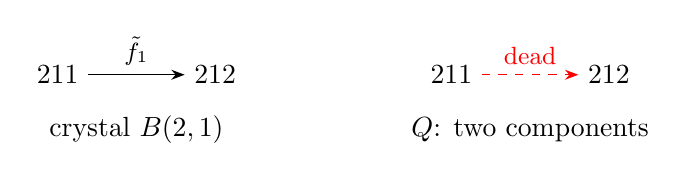
\begin{tikzpicture}[>=Stealth]
\node (a) at (0,0) {$211$}; \node (b) at (2,0) {$212$};
\draw[->] (a) -- node[above]{\small $\tf_1$} (b);
\node at (1,-0.7) {crystal $B(2,1)$};
\node (c) at (5,0) {$211$}; \node (d) at (7,0) {$212$};
\draw[->,dashed,red] (c) -- node[above]{\small dead} (d);
\node at (6,-0.7) {$Q$: two components};
\end{tikzpicture}
\end{center}
\emph{Non-example.} $Q$ is not ``delete edges between different standardisations'' applied to an arbitrary crystal. On a non-polynomial crystal such as $\det^{-1}$ (one point, weight $(-1,-1)$, $\teps=0$), the point is dead ($\delta_1=-1$) although it has no edge at all.
\end{example}

%======================================================================
\section{The defect identity and the quasi-tensor rule}

\begin{definition}[quasi-tensor product, word order]\label{def:qt}
For quasi-crystals $Q,Q'$, let $Q\qt Q'=Q\times Q'$ with additive weight, and for each $i$:
\begin{itemize}
\item $\eps_i(x\qt y)=\vphi_i(x\qt y)=\infty$ (and $\ee_i=\ff_i=\bot$) iff $\eps_i(x)=\infty$ or $\eps_i(y)=\infty$ or $\big(\eps_i(x)>0$ and $\vphi_i(y)>0\big)$. This last clause is the \emph{kill clause};
\item otherwise $\eps_i=\eps_i(x)+\eps_i(y)$ and $\vphi_i=\vphi_i(x)+\vphi_i(y)$. $\ee_i$ acts on $x$ if $\eps_i(x)>0$, else on $y$ if $\eps_i(y)>0$, else gives $\bot$. $\ff_i$ acts on $y$ if $\vphi_i(y)>0$, else on $x$ if $\vphi_i(x)>0$, else gives $\bot$.
\end{itemize}
This is CGM's quasi-tensor product [2301.00271 Thm~5.1, Prop.~5.9, Def.~6.9] with factors reversed (see \S1).
\end{definition}

\begin{proposition}[defect identity]\label{prop:defect}
For seminormal $B,B'$ and any weights,
\[\boxed{\ \delta_i(x\otimes y)=\delta_i(x)+\delta_i(y)+\min\big(\teps_i(x),\tphi_i(y)\big).\ }\]
On words, the three terms count the brackets inside $u$, the brackets inside $v$, and the brackets crossing the cut (Lemma~\ref{lem:concat}).
\end{proposition}
\begin{proof}
$\wt_{i+1}$ is additive, and $\teps_i(x\otimes y)=\teps_i(x)+\teps_i(y)-\min(\teps_i(x),\tphi_i(y))$. Subtract.
\end{proof}

\begin{theorem}[quasification is strict monoidal; Q66]\label{thm:Q66}
Let $B,B'$ be seminormal crystals whose weights are all polynomial. Then the identity of $B\times B'$ is an equality of quasi-crystals
\[Q_{B\otimes B'}=Q_B\qt Q_{B'} .\]
\end{theorem}
\begin{proof}
Fix $i$, $x\in B$, $y\in B'$, and write $\varepsilon=\teps_i(x)$, $\varphi'=\tphi_i(y)$. By Lemma~\ref{lem:defect}(b) all three terms of the defect identity are $\ge0$, so
\[x\otimes y\text{ alive}\iff\delta(x)=0\ \wedge\ \delta(y)=0\ \wedge\ \min(\varepsilon,\varphi')=0.\]
\emph{Dead sets agree.} If $x$ is dead, then $\eps(x)=\infty$ in $Q_B$ and Def.~\ref{def:qt} kills, as $Q_{B\otimes B'}$ does. The same holds for $y$. If both are alive, then $\eps(x)=\varepsilon$ and $\vphi(y)=\varphi'$ by Lemma~\ref{lem:defect}(c), and ``$\min(\varepsilon,\varphi')>0$'' is exactly the kill clause. On the dead set both sides have $\eps=\vphi=\infty$ and $\ee=\ff=\bot$.
\emph{Alive set.} Here $m=0$, so $\teps(x\otimes y)=\varepsilon+\teps(y)=\eps(x)+\eps(y)$, and likewise for $\tphi$. The signature rule applies $\te$ to $x$ iff $\varepsilon>\varphi'$. Since $m=0$, either $\varepsilon=0$, in which case it acts on $y$ (or both rules give $\bot$), or $\varphi'=0<\varepsilon$, in which case it acts on $x$. That is the $\qt$ rule ``on $x$ if $\eps(x)>0$, else on $y$''. On the left, $\ee=\te$ because $x\otimes y$ is alive. On the right, $\ee$ applied to the alive factor is $\te$. The $\ff$ case is symmetric, using Lemma~\ref{lem:defect}(c).
\end{proof}

\begin{theoremA}[quasi-tensor rule on words; owner: Cain--Guilherme--Malheiro]\label{thm:A}
For all words $u\in[n]^m$, $v\in[n]^k$, the map $(u,v)\mapsto uv$ is an isomorphism of word quasi-crystals $[n]^m\qt[n]^k\cong[n]^{m+k}$. Explicitly: $uv$ has an $i$-inversion iff $u$ does, or $v$ does, or ($\eps_i(u)>0$ and $\vphi_i(v)>0$). Otherwise $\eps,\vphi$ add, $\ee_i$ acts on the leftmost factor containing an $i+1$, and $\ff_i$ acts on the rightmost factor containing an $i$.
\end{theoremA}
\begin{proof}[Proof (as a corollary)]
Word crystals have polynomial weights. By Lemma~\ref{lem:concat}, $[n]^{m+k}\cong[n]^m\otimes[n]^k$ as crystals, and quasification commutes with isomorphisms. Apply Theorem~\ref{thm:Q66} and Lemma~\ref{lem:defect}(e).
\end{proof}
\begin{proof}[Direct proof (PROVE 275)]
A subsequence $(i+1)\cdots i$ of $uv$ lies in $u$, in $v$, or straddles the cut. For inversion-free $u,v$, straddling means $u$ contains $i+1$ and $v$ contains $i$, i.e.\ $\eps(u)>0$ and $\vphi(v)>0$. Otherwise the subword is $i^{\vphi(u)}(i+1)^{\eps(u)}i^{\vphi(v)}(i+1)^{\eps(v)}$ with $\eps(u)\vphi(v)=0$, i.e.\ $i^{\vphi(u)+\vphi(v)}(i+1)^{\eps(u)+\eps(v)}$. Its leftmost $i+1$ is in $u$ iff $\eps(u)>0$.
\end{proof}

\begin{remark}[restating compresses]
In PROVE 275, Theorem A was proved first and Q66 (PROVE 276) afterwards. In dependency order Theorem A is the special case $B=[n]^m$, $B'=[n]^k$ of Q66. The kill clause \emph{is} the cross-cut term $\min(\teps(x),\tphi(y))$ of the defect identity. So the quasi-tensor rule is the Kashiwara signature rule restricted to pairs with no bracket across the cut. The asymmetry of the kill clause ($\eps(u)>0,\vphi(v)>0$ kills, while $\vphi(u)>0,\eps(v)>0$ is harmless) is the asymmetry of bracketing: an $i+1$ matches a \emph{later} $i$.
\end{remark}

\begin{example}
$n=2$, $i=1$. Take $u=2$, $v=1$: $\eps(u)=1$ and $\vphi(v)=1$, so the kill clause fires and $21$ is dead (one bracket, crossing the cut). Take $u=1$, $v=2$: no kill, and $12$ has $\eps=\vphi=1$, $\ee_1(12)=11$, $\ff_1(12)=22$.
\end{example}

\begin{example}[sharpness: polynomiality is needed]\label{ex:sharp}
(i) $\mathfrak{gl}_2$, $B=\det^{-1}$ (one point, weight $(-1,-1)$) and $B'=\det$ (one point, weight $(1,1)$). Then $\teps=\tphi=0$, $\delta=-1$ and $+1$, so both points are dead, and $Q_B\qt Q_{B'}$ has $\eps_1=\infty$. But $B\otimes B'$ has weight $(0,0)$, $\delta=0$, so $Q_{B\otimes B'}$ has $\eps_1=0$. The defects cancelled.
(ii) A lost edge: $B=B(0,-1)$ (weights $(0,-1)\to(-1,0)$, $\delta\equiv-1$) and $B'=B(2,1)$ ($\delta\equiv+1$). Then $B\otimes B'\supset B(2,0)$, whose $3$-element $1$-string (weights $(2,0),(1,1),(0,2)$) is alive in $Q_{B\otimes B'}$ with $\eps_1=0,1,2$. Every element of $Q_B\qt Q_{B'}$ is dead.
\end{example}

%======================================================================
\section{Components are standardisation classes (Theorem B)}

\begin{definition}
$\std(w)\in S_N$ labels the letters of $w$ by $1,\dots,N$, smallest letters first and equal letters left to right. For $\sigma\in S_N$ (as a word), $\iDes(\sigma)=\{k:k+1\text{ appears left of }k\}$. For $D\subseteq[N-1]$, let $P_D(n)=\{b_1\le\cdots\le b_N\text{ in }[n]: b_k<b_{k+1}\ \forall k\in D\}$, and
\[F_{N,D}(x_1,\dots,x_n)=\sum_{b\in P_D(n)}x_{b_1}\cdots x_{b_N}\]
(Gessel's fundamental quasisymmetric function). We write $F_\alpha$, where $\alpha$ is the composition of $N$ with partial sums $D$. $C_\sigma:=\{w\in[n]^N:\std w=\sigma\}$.
\end{definition}

\begin{lemma}[Gessel's bijection]\label{lem:gessel}
For $\sigma\in S_N$ with $D=\iDes\sigma$, the map $w\mapsto b$, $b_k:=$ the letter carrying label $k$ (i.e.\ $b_k=w_{\sigma^{-1}(k)}$, where $\sigma^{-1}(k)$ is the position of $k$ in $\sigma$), is a bijection $C_\sigma\to P_D(n)$ with $x^w=x_{b_1}\cdots x_{b_N}$. Hence $\operatorname{ch}C_\sigma=F_{\iDes\sigma}$.
\end{lemma}
\begin{proof}
Labels increase with letters, so $b$ is weakly increasing. If $b_k=b_{k+1}$, the labels $k,k+1$ sit on equal letters, which are labelled left to right, so $k$ is left of $k+1$ and $k\notin D$. Conversely, given $b\in P_D(n)$, put $w_{\sigma^{-1}(k)}=b_k$. The labels carried by a given value $c$ form an interval $[p,q]$ with $[p,q-1]\cap D=\varnothing$. So in $\sigma$ the entries $p,\dots,q$ appear left to right, and $\std$ labels the $c$'s exactly that way. Smaller values carry smaller labels, so $\std w=\sigma$. The two maps are inverse.
\end{proof}

\begin{theoremB}[components; content Gessel / CMRR / Krob--Thibon]
The connected components of the word quasi-crystal $[n]^N$ are exactly the nonempty $C_\sigma$. In $b$-coordinates $C_\sigma\cong P_D(n)$, and $P_D(n)$ has a unique $\ee$-source $b^0$, $b^0_k=1+|D\cap[1,k-1]|$, of weight $(\alpha_1,\dots,\alpha_\ell,0,\dots,0)$. Its character is $F_\alpha(x_1,\dots,x_n)$. $C_\sigma\ne\varnothing$ iff $\ell(\alpha)\le n$.
\end{theoremB}
\begin{proof}
\emph{(1) The operators in $b$-coordinates.} Let $w\in C_\sigma$, let $l$ be the number of letters $\le i$, and suppose $w$ contains an $i+1$, so $b_{l+1}=i+1$. Labels on equal letters increase left to right, so the leftmost $i+1$ carries label $l+1$. \emph{Claim:} $w$ is $i$-alive iff $l\notin D$ or there is no $i$ (i.e.\ $b_l\ne i$). If some $i+1$ precedes some $i$, then the first $i+1$ (label $l+1$) precedes the last $i$ (label $l$), so $l\in D$. Conversely, $l\in D$ with $b_l=i$ means label $l+1$ (an $i+1$) is left of label $l$ (an $i$). When alive, $\ee_i$ turns the leftmost $i+1$ into $i$. That letter becomes the rightmost $i$ (all $i$'s precede it), so every label is unchanged: $\std$ is preserved, and in $b$-coordinates $\ee_i$ lowers $b_{l+1}$ from $i+1$ to $i$. $\ff_i$ is the inverse partial map. So each $C_\sigma$ is a union of components.
\emph{(2) Connectedness and unique source.} By induction $b\ge b^0$ pointwise for $b\in P_D(n)$. Suppose $b\ne b^0$, let $k$ be minimal with $b_k>b^0_k$, and put $i+1:=b_k\ge2$. For $j<k$, $b_j=b^0_j\le b^0_k<b_k$, so $k$ is the first index with value $i+1$, i.e.\ $k=l+1$. If $b_{k-1}=i$, then $k-1\notin D$, since otherwise $b^0_k=b^0_{k-1}+1=b_{k-1}+1=b_k$. So by (1), $\ee_i$ applies (lowering $b_k$ to $i$ stays inside $P_D(n)$) and $\sum b$ drops. Iterating reaches $b^0$, so $P_D(n)$ is connected. $b^0$ admits no $\ee_i$, because the result would be $<b^0$ somewhere, contradicting $b\ge b^0$. So $b^0$ is the unique $\ee$-source. Its weight: $b^0$ takes value $j$ on the $j$-th block of $\alpha$. Nonempty iff $b^0_N=1+|D|\le n$.
\emph{(3)} The character is Lemma~\ref{lem:gessel}.
\end{proof}

\begin{example}[$C_{21}$ in $n=3$]
$\sigma=21$, $D=\{1\}$, $\alpha=(1,1)$: $C_{21}=\{21,31,32\}$ with
\begin{center}
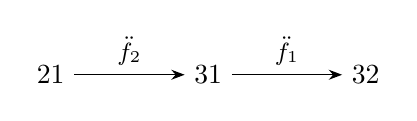
\begin{tikzpicture}[>=Stealth]
\node (a) at (0,0) {$21$}; \node (b) at (2,0) {$31$}; \node (c) at (4,0) {$32$};
\draw[->] (a) -- node[above]{\small$\ff_2$} (b); \draw[->] (b) -- node[above]{\small$\ff_1$} (c);
\end{tikzpicture}
\end{center}
Source $21$ has weight $(1,1,0)=\alpha$ padded. The character is $x_1x_2+x_1x_3+x_2x_3=F_{11}=e_2$. Here $21$ is $1$-dead and $32$ is $2$-dead. (Here $Q$ changes nothing relative to the crystal $B(1,1)$. Example~\ref{ex:211} is the smallest case where it does.)
\end{example}

%======================================================================
\section{Products: $K_0(\cQ_n)\cong\QSym_n$ as rings (Krob--Thibon; Q65)}

\begin{proposition}[the tensor shadow is the product]\label{prop:P}
For $\sigma_1\in S_m$, $\sigma_2\in S_k$: $\{uv:u\in C_{\sigma_1},v\in C_{\sigma_2}\}=\bigsqcup_{\tau\in\sigma_1\Cup\sigma_2}C_\tau$, where $\sigma_1\Cup\sigma_2=\{\tau\in S_{m+k}:\std(\tau_1\cdots\tau_m)=\sigma_1,\ \std(\tau_{m+1}\cdots\tau_{m+k})=\sigma_2\}$. Hence $F_{\iDes\sigma_1}F_{\iDes\sigma_2}=\sum_{\tau}F_{\iDes\tau}$.
\end{proposition}
\begin{proof}
$\std(u)$ and $\std(v)$ are the standardisations of the restrictions of $\std(uv)$ to the two position blocks. Conversely, a word $w$ with $\std w=\tau\in\sigma_1\Cup\sigma_2$ splits as $u\,v$ with $\std u=\sigma_1$, $\std v=\sigma_2$. For characters, use Lemma~\ref{lem:gessel} and additivity of weight.
\end{proof}

\begin{example}
$\sigma_1=1$, $\sigma_2=12$: $\sigma_1\Cup\sigma_2=\{123,213,312\}$ with $\iDes=\varnothing,\{1\},\{2\}$. So $F_1F_2=F_3+F_{12}+F_{21}$, and $C_{1}\qt C_{12}\cong C_{123}\sqcup C_{213}\sqcup C_{312}$.
\end{example}

\begin{definition}
$\cQ_n$ is the class of quasi-crystals isomorphic to finite disjoint unions of components of word quasi-crystals $[n]^N$, $N\ge0$. $K_0(\cQ_n)$ is the free abelian group on isoclasses of connected objects, with $[A\sqcup B]=[A]+[B]$, and multiplication $[Q][Q']=[Q\qt Q']$. $\QSym_n$ is the ring of quasisymmetric polynomials in $x_1,\dots,x_n$.
\end{definition}

\begin{lemma}\label{lem:basis}
$\{F_\alpha(x_1,\dots,x_n):\ell(\alpha)\le n\}$ is a $\mathbb Z$-basis of $\QSym_n$ (in particular, no repeats).
\end{lemma}
\begin{proof}
$F_\alpha=\sum_{\beta\text{ refines }\alpha}M_\beta$. In $n$ variables $M_\beta=0$ if $\ell(\beta)>n$. Otherwise $M_\beta$ has coefficient $1$ on $x^{(\beta,0,\dots)}$, and distinct $M_\beta$ have disjoint supports, so $\{M_\beta:\ell(\beta)\le n\}$ is a basis. The transition $F\to M$ is unitriangular for refinement.
\end{proof}

\begin{theorem}[Krob--Thibon {\cite{KT4,KT5}}, in quasi-crystal language; our Q65]\label{thm:Q65}
\begin{enumerate}[label=(\roman*)]
\item $C\mapsto\operatorname{ch}C$ is a bijection from isoclasses of connected objects of $\cQ_n$ to $\{F_\alpha(x_1..x_n):\ell(\alpha)\le n\}$.
\item $\cQ_n$ is closed under $\qt$, and $\operatorname{ch}(Q\qt Q')=\operatorname{ch}Q\cdot\operatorname{ch}Q'$. Hence $K_0(\cQ_n)\cong\QSym_n$ as rings, with isoclasses $\mapsto$ the $F$-basis.
\item (Commutativity for free.) $Q\qt Q'\cong Q'\qt Q$ for $Q,Q'\in\cQ_n$, although $\qt$ is not symmetric pointwise.
\item (Stability.) Let $\mathrm{res}:\cQ_{n+1}\to\cQ_n$ keep $\{\wt_{n+1}=0\}$ and forget index $n$. It commutes with $\qt$ and induces $x_{n+1}\mapsto0$. The inverse limit is $\QSym$, with $[C_\alpha]\mapsto F_\alpha$.
\end{enumerate}
\end{theorem}
\begin{proof}[Proof in our language]
(i) By Theorem B every connected object is $\cong P_D(n)$, and $P_D(n)$ depends only on $\alpha$. So the isoclass is a function of $\alpha$, and every $\alpha$ with $\ell(\alpha)\le n$ occurs. Injectivity: the weight of the unique $\ee$-source is $\alpha$ padded, and isomorphisms preserve sources and weights. (Alternatively, use Lemma~\ref{lem:basis}.)
(ii) Def.~\ref{def:qt} is pointwise in the factor data, so $\qt$ respects isomorphisms and distributes over $\sqcup$. For $Q\subseteq[n]^m$ and $Q'\subseteq[n]^k$ unions of components, Theorem A identifies $Q\qt Q'$ with $\{uv\}\subseteq[n]^{m+k}$. By Prop.~\ref{prop:P} this is a union of components. The unit is $\{\varnothing\}$, and associativity comes from concatenation. Weight is additive, so the character is multiplicative. Decomposition into components is canonical, so $K_0$ is free on connected isoclasses, which by (i) and Lemma~\ref{lem:basis} map bijectively onto a basis.
(iii) Both sides lie in $\cQ_n$ and have the same character because $\QSym_n$ is commutative. By (i) the character determines the isoclass of each component, and multiplicities are read off the $F$-expansion.
(iv) $\{\wt_{n+1}=0\}$ is closed under $\ee_i,\ff_i$ for $i<n$, and on words it is the set of words over $[n]$, so $\mathrm{res}\,C^{[n+1]}_\sigma=C^{[n]}_\sigma$. Weights are $\ge0$, so $\wt_{n+1}(x\qt y)=0$ iff both are $0$, and the $\qt$ rule for $i<n$ uses only $i$-data. Finally $F_\alpha(x_1..x_{n+1})|_{x_{n+1}=0}=F_\alpha(x_1..x_n)$.
\end{proof}

\begin{remark}[what Krob--Thibon prove, and what is assembled here]\label{rem:KT}
Krob and Thibon work with the degenerate quantum group at $q=0$: comodules over $A_0(n)$ in \cite{KT4}, and modules over $U_0(\mathfrak{gl}_N)$, obtained by putting $q=0$ in a variant of $U_q(\mathfrak{gl}_N)$, in \cite{KT5}. Precisely:
\begin{itemize}[leftmargin=*]
\item \cite[Prop.~6.1(2), p.~366]{KT4}: characters are multiplicative, $\chi(M\otimes N)=\chi(M)\chi(N)$ (for $A_q(n)$-comodules, any $q$).
\item \cite[Conj.~6.13, Note~6.14, p.~371]{KT4}: if the $D_I$ are a complete system of irreducible $A_0(n)$-comodules, then the character ring $\mathrm{Char}_{\mathbb Z}(0;n)$ is isomorphic to the $\mathbb Z$-algebra of quasi-symmetric functions in $n$ letters. This is conjectural in \cite{KT4}.
\item \cite[Prop.~7.1]{KT5}: $D_I$ is an irreducible $U_0(\mathfrak{gl}_N)$-module with character $F_I(x_1,\dots,x_N)$. In its proof they define the \emph{quasi-crystal graph} $N(I)$ on quasi-ribbon words of shape $I$ (the term is theirs), show that its arrows are Kashiwara's $\tilde e_i,\tilde f_i$ restricted to quasi-ribbon words, and show that $N(I)$ is strongly connected. This is the content of Theorem~B for the canonical representatives.
\item \cite[Prop.~7.3(i)]{KT5}: the $D_I$ form a complete family of irreducible polynomial $U_0(\mathfrak{gl}_N)$-modules. The closing remark of \cite[\S7]{KT5} then says that the commutative algebra spanned by the noncommutative quasi-ribbon functions is isomorphic to $\QSym$ and ``plays therefore the r\^ole of the character ring of polynomial $U_0(\mathfrak{gl}_N)$-modules''. The conference version is \cite{KTfpsac}.
\end{itemize}
Together these give, in substance, Theorem~\ref{thm:Q65}(i),(ii): irreducibles are indexed by compositions with characters $F_\alpha$, and the character ring is $\QSym_N$ with tensor product going to product. KT do not state it as one theorem; we assemble it from the propositions above. What is \emph{not} in \cite{KT4,KT5}: Cain--Malheiro quasi-crystals as abstract objects, the quasi-tensor product $\qt$ with its kill clause, any functor from crystals (or generic $U_q$-modules) to quasi-crystals, and the defect identity. \cite[p.~353]{KT4} explicitly contrasts the $q=0$ specialisation with Kashiwara's crystallization (``describes a truly degenerate case, rather than combinatorial aspects of the generic situation''). So the restatement above, with $\qt$ in place of the $U_0$ tensor product, uses Theorem~A, and the comparison with crystals in \S\ref{sec:sym} uses Theorem~\ref{thm:Q66}. Those are the parts that rest on the new identity.
\end{remark}

%======================================================================
\section{Branching: $\Res_a$ induces $\Delta$}

\begin{theorem}[Levi branching]\label{thm:C}
Fix $1\le a\le n-1$, and let $\Res_a$ forget $\ee_a,\ff_a$. Read the result as an $A_{a-1}\times A_{n-a-1}$ quasi-crystal, with letters $\le a$ in the first factor and letters $>a$ (shifted down by $a$) in the second. For $C=C_\sigma$ with $D=\iDes\sigma$, $|\alpha|=N$:
\[\Res_aC_\sigma\cong\bigsqcup_{k=0}^N C^{(a)}_{\sigma_1^{(k)}}\boxtimes C^{(n-a)}_{\sigma_2^{(k)}},\]
where $\sigma^{(k)}_1=\std(\text{values }1..k\text{ of }\sigma\text{ in position order})$ and $\sigma^{(k)}_2$ is the same for the values $k+1..N$. Empty terms are dropped. $\iDes\sigma_1^{(k)}=D\cap[1,k-1]$ and $\iDes\sigma_2^{(k)}=(D\cap[k+1,N-1])-k$. Hence
\[\operatorname{ch}\Res_aC_\sigma=\sum_kF_{\beta_k}(x_{\le a})F_{\gamma_k}(x_{>a})=F_\alpha(x_{\le a};x_{>a})=(\Delta F_\alpha)(x_{\le a};x_{>a}),\]
with $\alpha=\beta_k\cdot\gamma_k$ if $k\in D\cup\{0,N\}$ and $\alpha=\beta_k\odot\gamma_k$ (last part of $\beta_k$ merged with first part of $\gamma_k$) if $k\notin D$.
\end{theorem}
\begin{proof}
Operators with $i\ne a$ never move a letter across $a\leftrightarrow a+1$, so $k=\#\{\text{letters}\le a\}$ is invariant. Fix $k$ and set $\psi(w)=(w|_{\le a},\,w|_{>a}-a)$ (subwords). For $i<a$, the operators and the inversion test see only letters $i,i+1\le a$, so $\psi$ intertwines them on the first coordinate and fixes the second. The case $i>a$ is symmetric. Since $\std w=\sigma$, the letters $\le a$ sit exactly at the positions of the values $1..k$ of $\sigma$, so $\psi$ is injective on the slice. It is surjective onto $C_{\sigma_1}\times C_{\sigma_2}$: put $u$ at those positions and $v+a$ elsewhere. Every letter of $u$ is below every letter of $v+a$, so the standardisation is $\sigma$. Each factor is connected (Theorem B), so each slice is one component of the product. For the $\iDes$ computation, the relative positions of $j,j+1$ within one value block are inherited from $\sigma$. The descent at $k$ itself is lost, and it is recorded in the choice $\cdot$ versus $\odot$. The final equality is the definition of $\Delta$ on the $F$-basis [Grinberg--Reiner 1409.8356, \S5], equivalently Gessel's $F_\alpha(x+y)$ formula.
\end{proof}

\begin{example}
$\alpha=(2,1)$, $D=\{2\}$. The cuts $k=0,1,2,3$ give $(\varnothing,21)$, $(1,11)$, $(2,1)$, $(21,\varnothing)$, so $\Delta F_{21}=1\otimes F_{21}+F_1\otimes F_{11}+F_2\otimes F_1+F_{21}\otimes1$.
\end{example}

\begin{corollary}
$\Res_a(Q\qt Q')=\Res_aQ\qt\Res_aQ'$, and $(A\boxtimes B)\qt(A'\boxtimes B')\cong(A\qt A')\boxtimes(B\qt B')$. Hence $\Res_a$ is a ring map $K_0(\cQ_n)\to K_0(\cQ_a)\otimes K_0(\cQ_{n-a})$, $f\mapsto f(x_{\le a};x_{>a})$. As $a,n-a\to\infty$ this is $\Delta:\QSym\to\QSym\otimes\QSym$, and its multiplicativity (the bialgebra axiom) is realised by quasi-crystals.
\end{corollary}
\begin{proof}
The $\qt$ rule is per index. For $i<a$ all the $i$-data of $(a,b)$ are those of $a$, so $((a,b),(a',b'))\mapsto((a,a'),(b,b'))$ is the isomorphism.
\end{proof}

%======================================================================
\section{Crystals $\to$ quasi-crystals: $\Sym_n\hookrightarrow\QSym_n$}\label{sec:sym}

\begin{corollary}\label{cor:sym}
\begin{enumerate}[label=(\alph*)]
\item $Q_{B(\lambda)}\in\cQ_n$ and $\operatorname{ch}Q_{B(\lambda)}=s_\lambda$.
\item $[B]\mapsto[Q_B]$ is an injective ring map $\Sym_n=K_0(\text{polynomial }\mathfrak{gl}_n\text{ crystals})\to K_0(\cQ_n)=\QSym_n$. Under $\operatorname{ch}$ it is the inclusion $\Sym_n\subset\QSym_n$.
\item $[Q_{B(\lambda)}]=\sum_{T\in SYT(\lambda)}[C_{\mathrm{Des}T}]$, so $Q$ splits $B(\lambda)$ into $f^\lambda$ quasi-components (CMRR2 Cor.~4.10).
\item $\Res_a\circ Q=Q\circ\Res_a$.
\end{enumerate}
\end{corollary}
\begin{proof}
(a) Black box~\ref{bb:Blambda} realises $B(\lambda)$ as a component of $[n]^N$. Quasification is pointwise, so $Q$ of a subcrystal is the restriction of $Q_{[n]^N}$, which is the word quasi-crystal (Lemma~\ref{lem:defect}(e)). The restriction is closed under $\ee,\ff$, hence is a union of quasi-components. The set and weights are unchanged.
(b) Additivity is clear. Multiplicativity is Theorem~\ref{thm:Q66} (Black box~\ref{bb:tensor}). $\operatorname{ch}Q_B=\operatorname{ch}B$, so the map is the inclusion.
(c) Theorem~\ref{thm:Q65}(i) forces $[Q_{B(\lambda)}]=\operatorname{ch}^{-1}(s_\lambda)$. Now expand by Black box~\ref{bb:gessel}.
(d) Def.~\ref{def:Q} is per index.
\end{proof}

\begin{example}
In $\mathfrak{gl}_2$, $B(2,1)$ is the 2-element crystal of Example~\ref{ex:211}, and $s_{21}(x_1,x_2)=F_{12}+F_{21}$: two quasi-components. In $\mathfrak{gl}_3$, $s_{21}=F_{12}+F_{21}$ again, and the $x_1x_2x_3$ coefficient is $2=1+1$.
\end{example}

%======================================================================
\section{Punchline: tensor $\leftrightarrow$ product, branching $\leftrightarrow$ coproduct}

\begin{center}
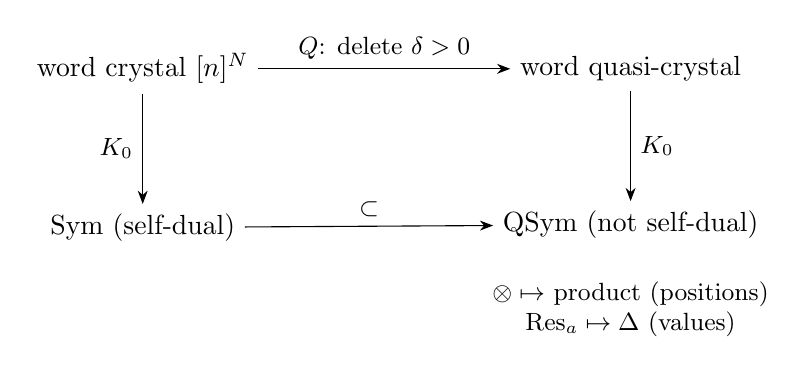
\begin{tikzpicture}[>=Stealth,node distance=1.4cm and 3.2cm]
\node (wc) {word crystal $[n]^N$};
\node (qc) [right=of wc] {word quasi-crystal};
\node (sym) [below=of wc] {$\Sym$ (self-dual)};
\node (qsym) [below=of qc] {$\QSym$ (not self-dual)};
\draw[->] (wc) -- node[above]{\small $Q$: delete $\delta>0$} (qc);
\draw[->] (wc) -- node[left]{\small $K_0$} (sym);
\draw[->] (qc) -- node[right]{\small $K_0$} (qsym);
\draw[->] (sym) -- node[above]{\small $\subset$} (qsym);
\node[below=0.3cm of qsym,align=center,font=\small] {$\otimes\mapsto$ product (positions)\\ $\Res_a\mapsto\Delta$ (values)};
\end{tikzpicture}
\end{center}

\begin{enumerate}[leftmargin=*]
\item \textbf{Two operations, not one.} Seed Path 4 asks why the $\Sym$ coproduct matches both the crystal tensor rule and restriction. It doesn't match both. Tensor products shadow the \emph{product} (Prop.~\ref{prop:P}, the restriction of $\sigma$ to \emph{position} blocks). Branching shadows the \emph{coproduct} (Theorem~\ref{thm:C}, the restriction of $\sigma$ to \emph{value} blocks). In $\Sym$ both give $c^\lambda_{\mu\nu}$ because $\Sym$ is self-dual. In $\QSym$ they separate. Minimal separator: $C_{312}$ (character $F_{21}$) is a component of $C_1\qt C_{12}$, yet $F_1\otimes F_2$ does not occur in $\Delta F_{21}$.
\item \textbf{Zero-cross-cut-bracket locus.} By the defect identity, quasification is the locus with no bracket inside either factor and none across the cut. The crystal keeps the cross-cut bracket and pays with a non-strict (bracketed) tensor rule. The quasi-crystal deletes it, which makes the tensor rule factor-local for every cut, and pays with self-duality.
\item \textbf{Positions $\leftrightarrow$ values.} These two restrictions are swapped by $\sigma\leftrightarrow\sigma^{-1}$. The components $C_\sigma$ remember all of $\sigma$, so they live at the level of $\mathrm{FQSym}$, whose self-duality $F_\sigma\leftrightarrow G_{\sigma^{-1}}$ (Malvenuto--Reutenauer) is the plausible home of this swap. \emph{Grade: hunch, interpretive, not proved here.}
\item \textbf{Seed Q1 / Q4.} $\QSym$ is the terminal combinatorial Hopf algebra (Aguiar--Bergeron--Sottile). Its ``$q=0$'' categorical avatar is a crystal-like graph, the type-$A$ quasi-crystal, just as $B(\lambda)$ is for $\Sym=K_0(\mathrm{Rep}\,U_q(\mathfrak{gl}_\infty))$. The inclusion $\Sym\subset\QSym$ is the $K_0$-shadow of the forgetful functor $Q$, i.e.\ of ``a crystal is a union of quasi-crystals''. This is a bialgebra-level statement only. The antipode and the ABS character $\zeta$ have \emph{not} been given categorical meaning.
\end{enumerate}

%======================================================================
\section{Who owns what}\label{sec:owners}

\begin{itemize}[leftmargin=*]
\item Word quasi-crystals and quasi-Kashiwara operators: Cain--Malheiro (hypoplactic monoid), in the convention of Cain--Malheiro--F.~Rodrigues--I.~Rodrigues [CMRR1 2309.14887 Def.~2.13]. Quasification: [CMRR2 2309.14898 Def.~4.5]. The $f^\lambda$ count: [CMRR2 Cor.~4.10].
\item Quasi-tensor product and Theorem A: Cain--Guilherme--Malheiro [2301.00271 Thm~5.1, Prop.~5.9, Def.~6.9], with word reversal.
\item Theorem B, Prop.~\ref{prop:P}, Theorem~\ref{thm:C} (content): Gessel 1984; Malvenuto--Reutenauer 1995 (shuffle product, $F_\alpha(x+y)$); Krob--Thibon \cite{KT4,KT5} (quasi-symmetric functions, $0$-Hecke algebras, and the quasi-crystal graph $N(I)$ of \cite[\S7]{KT5}).
\item Theorem~\ref{thm:Q65} ($K_0\cong\QSym_n$ as rings, tensor $\mapsto$ product): Krob--Thibon, in substance, in the language of polynomial $U_0(\mathfrak{gl}_N)$-modules \cite[Prop.~6.1, Conj.~6.13, Note~6.14]{KT4}, \cite[Props.~7.1, 7.3]{KT5}; see Remark~\ref{rem:KT}. Ours: only the restatement for Cain--Malheiro quasi-crystals with $\qt$, and the stability and commutativity remarks (iii),(iv), which are immediate.
\item The defect identity (Proposition~\ref{prop:defect}) and Theorem~\ref{thm:Q66} (quasification is strict monoidal), with Theorem~A re-derived from it and Corollary~\ref{cor:sym}(b): we did not find these stated in Krob--Thibon \cite{KT4,KT5}, Maas-Gari\'epy 2302.07694, Brauner--Corteel--Daugherty--Schilling 2503.14782, CMRR 2309.14887/2309.14898, Brauner--Daugherty--Mason--Schilling 2607.12232, Kobayashi 2512.06273, or Appleby--Simone--McGinley 2610.33772. This check covers only these sources, and the absence of a statement there is not evidence of novelty. This is the part of the note we regard as new.
\end{itemize}

%======================================================================
\section{Open questions}
\begin{enumerate}[leftmargin=*]
\item \textbf{Intrinsic characterisation.} $\cQ_n$ is defined via words. Do CMRR's local axioms for quasi-crystals (2309.14898) characterise the objects of $\cQ_n$? A yes makes Theorem~\ref{thm:Q65} axiomatic. A no would be an axiom-satisfying quasi-crystal not isomorphic to any $P_D(n)$.
\item \textbf{Antipode and $\zeta$.} Is there a categorical meaning (a duality on $\cQ_n$, a ``sign'' or reversal functor) inducing the antipode of $\QSym$, or the ABS character $\zeta$? Partial: none.
\item \textbf{Cross-cut brackets and self-duality.} Does the cross-cut bracket ``cause'' the self-duality of $\Sym$ (RSK)? No separator has been proposed. This is interpretive.
\item \textbf{Other kill rules (closed, empty).} The opposite kill clause ($\vphi(x)>0\wedge\eps(y)>0$), with the operator choices mirrored, is our rule applied to the swapped pair $(y,x)$. That is the opposite monoidal structure $Q\qt^{\mathrm{op}}Q':=Q'\qt Q$. Its $K_0$ is the same commutative ring. So the swapped-order control (which fails) shows a \emph{different} rule, not a different category.
\end{enumerate}

\begin{thebibliography}{KT99}
\bibitem[KT97]{KT4} D.~Krob and J.-Y.~Thibon, \emph{Noncommutative symmetric functions IV: Quantum linear groups and Hecke algebras at $q=0$}, J.\ Algebraic Combin.\ \textbf{6} (1997), 339--376.
\bibitem[KT99]{KT5} D.~Krob and J.-Y.~Thibon, \emph{Noncommutative symmetric functions V: a degenerate version of $U_q(\mathfrak{gl}_N)$}, Internat.\ J.\ Algebra Comput.\ \textbf{9} (1999), 405--430.
\bibitem[KTf]{KTfpsac} D.~Krob and J.-Y.~Thibon, \emph{A crystalizable version of $U_q(\mathfrak{gl}_N)$}, extended abstract, Formal Power Series and Algebraic Combinatorics (FPSAC'97), Vienna, 1997. Conference version of \cite{KT5}.
\end{thebibliography}

\appendix
\section{Verification}
Every displayed example was re-implemented from the printed statements (\texttt{proofs/prove277/examples.py}, independent of the PROVE 275/276 code). Results: Theorem A rule versus the definition, $1272$ cases ($n\le4$, $|u|+|v|\le3$), $0$ failures; swapped kill clause, $6$ failures on $n=2$, $|u|=|v|=2$ (the control breaks); defect identity on words ($n=3$, $|u|=|v|=3$), $0$ failures; components $=\std$ classes ($n=3$, $N=4$); $C_{21}$ chain; $211$/$212$ dead; $F_1F_2=F_3+F_{12}+F_{21}$ ($n=4$); the shuffle set $\{123,213,312\}$; $\Delta F_{21}$ cuts; $\det^{-1}\otimes\det$ and $B(0,-1)\otimes B(2,1)$ as stated; Theorem B unique source of weight $\alpha$ padded ($N\le4$, $n\le4$, all $\sigma$), $0$ failures; Theorem~\ref{thm:C} ($\psi$ a bijection onto $C_{\sigma_1}\times C_{\sigma_2}$ and the $\iDes$ formulas) on $464$ slices, $0$ failures. Earlier larger runs: \texttt{proofs/prove275/}, \texttt{proofs/prove276/} (Q66: 134 tensor pairs, 5418 elements, 0 failures; control 4500 failures).

\end{document}
